\documentclass{standalone}
\usepackage{tikz}
\begin{document}
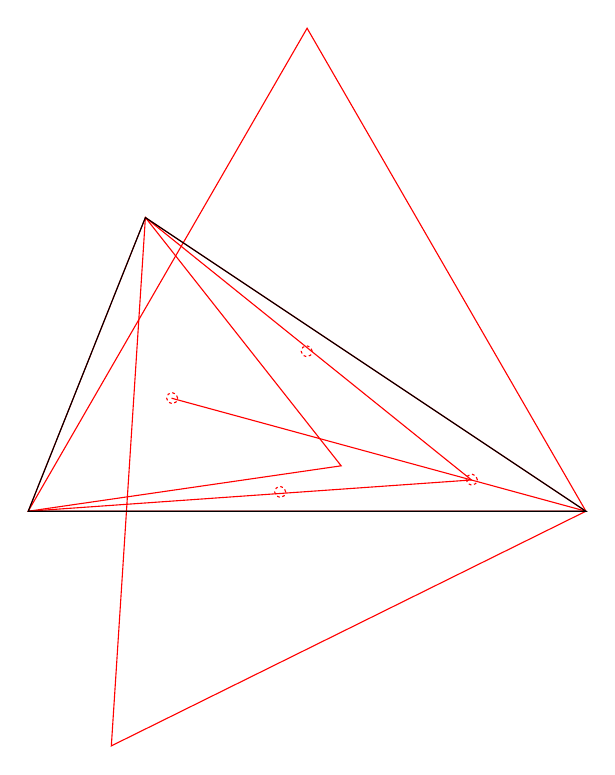
\begin{tikzpicture}[x=1pt,y=1pt]
\draw[red] (64.75,-88.71) -- (135.49,-178.43) -- (22.41,-194.84) -- cycle;
\draw[red] (52.44,-279.63) -- (223.94,-194.84) -- (64.75,-88.71) -- cycle;
\draw[red] (22.41,-194.84) -- (223.93,-194.84) -- (123.18,-20.31) -- cycle;
\draw[red] (223.93,-194.84) -- (74.22,-154.00);
\draw[red] (64.75,-88.71) -- (182.59,-183.55);
\draw[red] (22.41,-194.84) -- (182.59,-183.55);
\draw[red, dash pattern=on 1pt] (123.03,-137.03) circle (2.00);
\draw[red, dash pattern=on 1pt] (113.45,-187.86) circle (2.00);
\draw[red, dash pattern=on 1pt] (74.41,-153.97) circle (2.00);
\draw[red, dash pattern=on 1pt] (182.70,-183.44) circle (2.00);
\draw (22.41,-194.84) -- (223.93,-194.84) -- (64.75,-88.71) -- cycle;
\end{tikzpicture}
\end{document}
